\documentclass[a4paper, 14pt]{extarticle}
\usepackage{geometry}

\usepackage{cmap} % Улучшенный поиск русских слов в полученном pdf-файле
\usepackage{mathtext} % русские буквы в формулах
\defaulthyphenchar=127 % Если стоит до fontenc, то переносы не впишутся в выделяемый текст при 
%копировании его в буфер обмена
\usepackage[T2A]{fontenc}
\usepackage[utf8]{inputenc}
\usepackage[english, russian]{babel}
\usepackage{pscyr}  
\renewcommand{\rmdefault}{ftm} % ftm - (TimesNewRoman), fac - Academy, fad - Advertisement, flz - 
%Lazurski, fcr - CourierNewPSM, others in pscyr.sty

\usepackage{amsthm,amsfonts,amsmath,amssymb,amscd} % Математические дополнения от AMS
\usepackage{mathtools} % Добавляет окружение multlined

\usepackage{longtable} % Длинные таблицы
\usepackage{multirow,makecell,array} % Улучшенное форматирование таблиц
\usepackage{booktabs} % Возможность оформления таблиц в классическом книжном стиле

\usepackage{soulutf8} % Поддержка переносоустойчивых подчёркиваний и зачёркиваний
\usepackage{icomma} % Запятая в десятичных дробях

\usepackage[usenames,dvipsnames,svgnames,table,rgb]{xcolor}

\usepackage{hyperref}

\usepackage{graphicx} % Подключаем пакет работы с графикой
\graphicspath{{../images/}{images/}} % Пути к изображениям

%%% Подписи %%%
\usepackage[singlelinecheck=off,center]{caption}
\usepackage{subcaption}

\usepackage[onehalfspacing]{setspace}

%%% Списки %%%
\usepackage{enumitem}

%%% Библиография %%%
\usepackage{cite} % Красивые ссылки на литературу

%%% Оглавление %%%
\usepackage[nottoc]{tocbibind}
\usepackage{tocloft}
\usepackage{titlesec}

\usepackage{titlesec} % Растояние между заголовками и текстом
\usepackage{float}
\usepackage{listings} % Listings

\usepackage{lipsum}

\geometry{a4paper,top=2cm,bottom=2cm,left=2cm,right=1cm}
%%% Выравнивание и переносы %%%
\sloppy                             % Избавляемся от переполнений
\clubpenalty=10000                  % Запрещаем разрыв страницы после первой строки абзаца
\widowpenalty=10000                 % Запрещаем разрыв страницы после последней строки абзаца
\usepackage{indentfirst}
\frenchspacing
\setlength{\parindent}{2.5em} % Абзацный отступ
\linespread{1.3}

% colors
\definecolor{linkcolor}{rgb}{0.9,0,0}
\definecolor{citecolor}{rgb}{0,0.6,0}
\definecolor{urlcolor}{rgb}{0,0,1}
\definecolor{mygreen}{rgb}{0,0.6,0}
\definecolor{mygray}{rgb}{0.5,0.5,0.5}
\definecolor{mymauve}{rgb}{0.58,0,0.82}
\definecolor{myblack}{rgb}{0,0,0}

\hypersetup{				% Гиперссылки
    unicode=true,          % non-Latin characters in Acrobat’s bookmarks
    pdftoolbar=true,        % show Acrobat’s toolbar?
    pdfmenubar=true,        % show Acrobat’s menu?
    pdffitwindow=false,     % window fit to page when opened
    pdfstartview={FitH},    % fits the width of the page to the window
    pdftitle={Classification and Aggregation of News Articles Using Methods and Models of Natural Language Processing},    % title
    pdfauthor={Dmitry Yutkin, Vasily Vdovkin},     % author
    pdfsubject={Course work},   % subject of the document
    pdfcreator={Dmitry Yutkin, Vasily Vdovkin},   % creator of the document
    pdfproducer={Dmitry Yutkin, Vasily Vdovkin}, % producer of the document
    pdfkeywords={nlp}{text}{classification}{aggregation}{news}{articles}{svm}{rnn}{deep}{learning}
    {machine}{learning}{машинное}{глубокое}{обучение}{нейронные}{сети}{нлп}, % Ключевые слова
    pdfnewwindow=true,
    pdflang={ru},
    linktocpage=true,
    plainpages=false,
    colorlinks,       	    % false: ссылки в рамках; true: цветные ссылки
    linkcolor={linkcolor},      % цвет ссылок типа ref, eqref и подобных
    citecolor={citecolor},      % цвет ссылок-цитат
    urlcolor={urlcolor},        % цвет гиперссылок
}

%% Рисунки %%%
\DeclareCaptionLabelSeparator{emdash}{~--- }
\captionsetup[figure]{labelsep=emdash,font=onehalfspacing,position=bottom}
\captionsetup[subfigure]{subrefformat=simple,labelformat=simple}
\renewcommand\thesubfigure{(\alph{subfigure})}

\captionsetup{%
    singlelinecheck=off,                % Многострочные подписи, например у таблиц
    skip=2pt,                           % Вертикальная отбивка между подписью и содержимым рисунка или таблицы определяется ключом
    justification=centering,            % Центрирование подписей, заданных командой \caption
}

%% Подписи подрисунков %%%
\renewcommand{\thesubfigure}{\asbuk{subfigure}}           % Буквенные номера подрисунков
\captionsetup[subfigure]{font={normalsize},               % Шрифт подписи названий подрисунков (не отличается от основного)
    labelformat=brace,                                    % Формат обозначения подрисунка
    justification=centering,                              % Выключка подписей (форматирование), один из вариантов            
}

%%% Списки %%%
% Используем короткое тире (endash) для ненумерованных списков (ГОСТ 2.105-95, пункт 4.1.7, требует дефиса, но так лучше смотрится)
\renewcommand{\labelitemi}{\normalfont\bfseries{--}}

% Перечисление строчными буквами русского алфавита (ГОСТ 2.105-95, 4.1.7)
%\makeatletter
%    \AddEnumerateCounter{\asbuk}{\russian@alph}{щ}
%\makeatother
%\setlist[enumerate,1]{label=\asbuk{enumi})} % первого уровня 1), 2)...
%\setlist[enumerate,2]{label=\arabic*)} % второго уровня а), б) ... 

\setlist{nosep,%                                    % Единый стиль для всех списков (пакет enumitem), без дополнительных интервалов.
    labelindent=\parindent,leftmargin=*%            % Каждый пункт, подпункт и перечисление записывают с абзацного отступа
}

%%% Переопределение именований %%%
\addto\captionsrussian{%
    \renewcommand{\partname}{Часть}
    \renewcommand{\abstractname}{Аннотация}
    \renewcommand{\contentsname}{Оглавление} % (ГОСТ Р 7.0.11-2011, 4)
    \renewcommand{\figurename}{Рисунок} % (ГОСТ Р 7.0.11-2011, 5.3.9)
    \renewcommand{\tablename}{Таблица} % (ГОСТ Р 7.0.11-2011, 5.3.10)
    \renewcommand{\indexname}{Предметный указатель}
    \renewcommand{\listfigurename}{Список рисунков}
    \renewcommand{\listtablename}{Список таблиц}
}
%
%%% Старт отсчет страниц с титульника
\makeatletter
\renewenvironment{titlepage}
 {%
  \if@twocolumn
    \@restonecoltrue\onecolumn
  \else
    \@restonecolfalse\newpage
  \fi
  \thispagestyle{empty}%
 }
 {%
  \if@restonecol
    \twocolumn
  \else
    \newpage
  \fi
 }
\makeatother
%%%

%%% Библиография %%%
\makeatletter
\bibliographystyle{utf8gost71u}     % Оформляем библиографию по ГОСТ 7.1 (ГОСТ Р 7.0.11-2011, 5.6.7)
\renewcommand{\@biblabel}[1]{#1.}   % Заменяем библиографию с квадратных скобок на точку
\makeatother

%%% Оглавление %%%
\cftsetrmarg{2.55em plus1fil} %To have the (sectional) titles in the ToC, etc., typeset ragged right with no hyphenation
\renewcommand{\cftsecdotsep}{\cftdotsep} % отбивка точками до номера страницы начала главы/раздела
\renewcommand{\cftsecpagefont}{\normalfont}        % нежирные номера страниц у глав в оглавлении
\renewcommand{\cftsecleader}{\cftdotfill{\cftsecdotsep}}% нежирные точки до номеров страниц у глав в оглавлении
\renewcommand{\cfttoctitlefont}{\filright\fontsize{16pt}{18pt}\selectfont\bfseries} % Размер заголовка оглавления

%\renewcommand{\cftsecfont}{}                       % нежирные названия глав в оглавлении
%\renewcommand\cftsecaftersnum{.\ }   % добавляет точку с пробелом после номера раздела в оглавлении
%\renewcommand\cftsecaftersnum{.\ }    % добавляет точку с пробелом после номера подраздела в оглавлении
%\renewcommand\cftsubsecaftersnum{.\ } % добавляет точку с пробелом после номера подподраздела в оглавлении
%\renewcommand\cftsecaftersnum{\quad}     % добавляет \quad после номера раздела в оглавлении
%\renewcommand\cftsecaftersnum{\quad}      % добавляет \quad после номера подраздела в оглавлении
%\renewcommand\cftsubsecaftersnum{\quad}   % добавляет \quad после номера подподраздела в оглавлении
%\addtocontents{toc}{~\hfill{Стр.}\par}% добавить Стр. над номерами страниц

%%% Оформление заголовков глав, разделов, подразделов %%%
\titleformat{\section}[block]
    %{\filcenter\fontsize{16pt}{18pt}\selectfont\bfseries}{\thesection\cftsecaftersnum}{0.5em}{} % по центру
    {\filright\fontsize{16pt}{18pt}\selectfont\bfseries}{\thesection\cftsecaftersnum}{0.5em}{} % справа

\titleformat{\subsection}[block]
    %{\filcenter\fontsize{16pt}{18pt}\selectfont\bfseries}{\thesubsection\cftsubsecaftersnum}{0.5em}{}
    {\filright\fontsize{16pt}{18pt}\selectfont\bfseries}{\thesubsection\cftsubsecaftersnum}{0.5em}{}

\titleformat{\subsubsection}[block]
    %{\filcenter\fontsize{16pt}{18pt}\selectfont\bfseries}{\thesubsubsection\cftsubsecaftersnum}{0.5em}{}
    {\filright\fontsize{16pt}{18pt}\selectfont\bfseries}{\thesubsubsection\cftsubsecaftersnum}{0.5em}{}

%\renewcommand{\abstractnamefont}{\fontsize{16pt}{18pt}\selectfont\bfseries} % Размер заголовка аннтоации


% Расстояние между текстом и заголовками
%\setlength{\abstitleskip}{-25pt} % расстояние между заголовком аннтоации и тестом
\titlespacing{\section}{\parindent}{*2}{*1} % Расстояние между заголовком раздела и текстом должно быть равно удвоенному межстрочному интервалу.  Расстояние между основаниями строк заголовка принимают такими же, как в тексте
\titlespacing{\subsection}{\parindent}{*2}{*1}
\titlespacing{\subsubsection}{\parindent}{*2}{*1}

% Listings
\captionsetup[lstlisting]{labelsep=emdash}
\lstset{ %
  backgroundcolor=\color{white},   % choose the background color; you must add \usepackage{color} or \usepackage{xcolor}
  basicstyle=\ttfamily\footnotesize,        % the size of the fonts that are used for the code
  breakatwhitespace=false,         % sets if automatic breaks should only happen at whitespace
  breaklines=true,                 % sets automatic line breaking
  captionpos=t,                    % sets the caption-position to bottom
  commentstyle=\ttfamily,    % comment style
  columns=fixed,
  deletekeywords={...},            % if you want to delete keywords from the given language
  escapeinside={\%*}{*)},          % if you want to add LaTeX within your code
  extendedchars=true,              % lets you use non-ASCII characters; for 8-bits encodings only, does not work with UTF-8
  frame=none,	                   % adds a frame around the code
  keepspaces=true,                 % keeps spaces in text, useful for keeping indentation of code (possibly needs columns=flexible)
  keywordstyle=\ttfamily\bfseries,       % keyword style
  otherkeywords={*,...},           % if you want to add more keywords to the set
  numbers=left,                    % where to put the line-numbers; possible values are (none, left, right)
  numbersep=5pt,                   % how far the line-numbers are from the code
  numberstyle=\footnotesize\color{mygray}, % the style that is used for the line-numbers
  rulecolor=\color{black},         % if not set, the frame-color may be changed on line-breaks within not-black text (e.g. comments (green here))
  showspaces=false,                % show spaces everywhere adding particular underscores; it overrides 'showstringspaces'
  showstringspaces=false,          % underline spaces within strings only
  showtabs=false,                  % show tabs within strings adding particular underscores
  stepnumber=1,                    % the step between two line-numbers. If it's 1, each line will be numbered
  stringstyle=\ttfamily,     % string literal style
  tabsize=4,	                   % sets default tabsize to 2 spaces
  title=\lstname                   % show the filename of files included with \lstinputlisting; also try caption instead of title
  % stringstyle=\color{mymauve}\ttfamily,     % string literal style
  % keywordstyle=\ttfamily\color{blue},       % keyword style
  % commentstyle=\ttfamily\color{mygreen},    % comment style
} % Файл со стилями
\begin{document}
\begin{titlepage}
    \begin{center}
        ФЕДЕРАЛЬНОЕ ГОСУДАРСТВЕННОЕ АВТОНОМНОЕ
        
        ОБРАЗОВАТЕЛЬНОЕ УЧРЕЖДЕНИЕ ВЫСШЕГО ОБРАЗОВАНИЯ
        
       <<НАЦИОНАЛЬНЫЙ ИССЛЕДОВАТЕЛЬСКИЙ УНИВЕРСИТЕТ
       
       ''ВЫСШАЯ~ШКОЛА~ЭКОНОМИКИ''>>
       \vspace{1cm}
 
        \textbf{Московский институт электроники и математики}
        \vspace{1cm}

        Юткин Дмитрий Игоревич, группа БИВ-144
		
		Вдовкин Василий Алексеевич, группа БИВ-144
        \vspace{1cm}
        
        \textbf{Классификация и агрегация новостных статей, используя методы и модели обработки естественного языка}
        
%        \textbf{\MakeUppercase{Research of reinforcement learning algorithms using <<OpenAI Gym>>}}
        
        % \textbf{\MakeUppercase{The application of reinforcement learning for playing computer games}}
        % \textbf{The application of reinforcement learning for playing computer games in <<OpenAI Gym>>}
        \vspace{1cm}

        Междисциплинарная курсовая работа
        
        по направлению 09.03.01 Информатика и вычислительная техника 

        студента образовательной программы бакалавриата
        
        <<Информатика и вычислительная техника>>
        
    \end{center}
    \vspace{1cm}
    \begin{flushright}
        Студент~\rule{4cm}{.1pt}~Д.И.\,Юткин
        
        Студент~\rule{4cm}{.1pt}~В.А.\,Вдовкин
        
        \vspace{1cm}
        
        Руководитель

        старший преподователь

        Л.Л.\,Волкова
        
        \rule{4cm}{.1pt}
    \end{flushright}
    \vfill\center{Москва 2017 г.}
\end{titlepage} % Титульник
\titleformat{\section}[block]
{\centering\fontsize{16pt}{18pt}\selectfont\bfseries}{\thesection\cftsecaftersnum}{0.5em}{} % по центру

\section*{Аннотация}
В данной курсовой работе изучаются подходы к сбору, анализу, классификации и кластеризации текстовых данных.
В результате работы удалось собрать корпус новостей, состоящий более чем из 1 млн документов, применить
два подхода к классификации текстовых документов: линейный SVM и градиентный бустинг над деревьями,
а также KMeans и графовые алгоритмы к кластеризации новостей. Для демонстрации практической значимости исследуемых алгоритмов, был разработан 
веб-сервис, который в реальном времени агрегирует новости от различных СМИ, автоматически расставляет для них теги и объединяет в кластеры 
семантически близкие статьи.

\section*{Abstract}
The coursework is dedicated to research of mining, analysis, classification and clustering methods of text data.
As a result, a dataset with more than 1 million Russian news articles was collected. Two approaches for text classification were successfully 
applied: linear SVM and gradient boosted trees. For solving clustering problem KMeans and graph-based algorithms were utilized. In order to show a 
practical  appliance of the research methods, web-service was developed.
The web-service is able to aggregate and analyze text data in the real-time. Moreover, it automatically labels news articles
and cluster them by semantic similarity.

\titleformat{\section}[block]
{\raggedright\fontsize{16pt}{18pt}\selectfont\bfseries}{\thesection\cftsecaftersnum}{0.5em}{} % справа % Аннотация
\tableofcontents
 % Оглавление 
% Тут комменты по всему:

\section{Введение}
% Неможко публицистическое введение, чтобы хорошо читалось
% ибо кроме введения обычно ничего не читают
С каждым годом вычислительные мощности современных компьютеров и сервисов, 
предлагающие облачные вычисления, позволяют 
обрабатывать всё большие массивы данных. Благодаря этому происходит быстрое 
развитие алгоритмов анализа данных и машинного обучения. Результат работы 
этих алгоритмов можно увидеть в нашей повседневной жизни: 
сервисы прогноза погоды, которые предсказывают направление движения 
облаков, персонализированная реклама, подстраивающиеся под 
интересы пользователя, автомобили с автопилотом и т.д. --- в основе всех 
этих разработок лежат алгоритмы интеллектуального анализа данных и 
машинного обучения.

Одна из важнейших проблем, возникающая перед исследователями и 
разработчиками подобных систем, заключается в поиске данных для обучения моделей,
которые в будущем будут использоваться для анализа новой информации.

Решением данной проблемы являются тексты из сети Интернет.
Петабайты информации, записанной на естественном языке за последние несколько 
десятилетий, доступны любому исследователю. Книги, новостные статьи, блоги, посты в 
социальных сетях --- всё это является источником легкодоступных данных.

Именно поэтому обработка естественного языка (Natrual Language Processing, 
NLP) получила большое развитие. За последние несколько лет появилось множество 
специализированных библиотек и сервисов для анализа естественного языка. К таким сервисам, 
например, относится IBM Watson --- набор платных продуктов, предлагающий различные
инструменты работы с текстом: от извлечения важной информации и 
классификации, до его генерации. %https://www.ibm.com/watson/
Яркими примерами свободнораспространяемых библиотек являются: NLTK, Gensim, MyStem,
pymorphy и многие другие.

В данной работе решаются две задачи:
\begin{enumerate}
	\item классификация тем новостных статей;
	\item агрегация новостных статей по смысловой близости.
\end{enumerate} 
Для придания работе новизны и оригинальности задача решается для русскоязычных новостей.

Практическая значимость работы доказывается на примере реализации в виде веб-сервиса новостного агрегатора,
который в реальном времени, с помощью алгоритмов и подходов предложенных в данной работе,
обрабатывает публикации русскоязычных интернет-СМИ.

% Какие то общие слова, почему мы делаем этот агрегатор, какие у него будут функции.
\section{Цель и задачи курсовой работы}
Целью курсовой работы является разработка веб-сервиса, который:
\begin{enumerate}
	\item в реальном времени получает статьи из русскоязычных новостных источников;
	\item классифицирует полученные статьи по общим темам;
	\item агрегирует по схожести содержания статьи из различных источников.
\end{enumerate}
Агрегация и классификация основана на исследуемых в работе алгоритмы.

Для достижения поставленной цели, должны быть выполнены следующие задачи:
\begin{enumerate}
	\item Изучить методы и модели автоматической обработки текста и естественного языка;
	\item Собрать корпус новостных статей для обучения моделей;
	\item Исследовать и реализовать различные подходы к классификации и агрегации текстовых документов;
	\item Разработать back-end и front-end инфраструктуру сервиса.
\end{enumerate}

\section{Сбор и подготовка данных}
\subsection{Получение данных из новостных источников}
Для получения робастных моделей машинного обучения, требуется достаточно большой корпус новостных статей,
содержащий несколько сотен тысяч документов. Обычно существуют готовые коллекции текстов, но из-за выбранных 
ограничений к документам, а именно: новости на русском языке вместе с тег --- словом, описывающим тему 
документа, найти такой корпус не удалось, поэтому было принято решение собрать данные самостоятельно.

В качестве новостных источников были выбраны следующие популярные СМИ:
<<Газета.Ru>>, <<Lenta.ru>>, <<ТАСС>>, <<Новая Газета>>, <<ВЕДОМОСТИ>>, <<РИА Новости>> и <<СПОРТ-ЭКСПРЕСС>>.
Последнее было выбрано по причине малого количества спортивных новостей от других источников.

При анализе сайтов СМИ стало понятно, что они имеют схожую структуру: для отображения ссылок на статьи,
используются страницы со списком новостей (<<Лента новостей>>), по которым можно итерироваться,
изменяя параметры запросов, например, дату последней новости на странице или количество показанных статей.
Для извлечения данных из источников реализован набор алгоритмов, которые опираются на описанную структуру.

Стоит отметить, что во многих случаях для получения чистого текста приходится ждать ответа от сервера и обрабатывать 
HTML содержание страниц, что сильно замедляет работу, поэтому алгоритмы получения новостей одновременно обрабатывают
в параллельных процессах множество веб-страниц, что значительно ускоряет работу. Данные алгоритмы также используются в основном
web-сервисе для получения недавних новостей.

При формировании корпуса, все новостные статьи сопровождались различными метаданными: название СМИ, ссылка на статью,
дата публикации, тег и заголовок. В результате было получено более 1,1 млн. новостей с 1999 по 2017 год, многие из 
которых имели неправильно проставленные темы или не имели тем вовсе. Причин тому может быть несколько, например,
ошибки редакторов или технические ограничения веб-сайтов новостных агентств. Например, большинство новостей на сайте <<
Новой Газеты>> помечены тегом <<политика>>, что зачастую не совпадает с истинным содержанием статьи. После детального анализа тегов 
стало ясно, что относить новости к рубрикам редакторы стали только после определённого времени, а все уже имеющие 
статьи на сайте отнесли в <<политику>>. Некорректные данные пришлось удалить.

В итоговую выборку, которая в дальнейшем использовалась для обучения и тестирования алгоритмов,
вошло $133\,529$ статей, помеченных 32 различными тегами. Распределение СМИ и тем на отобранных данных отражено на 
рисунке \ref{media_topic_distr}.
\begin{figure}[h!]
	\centering
	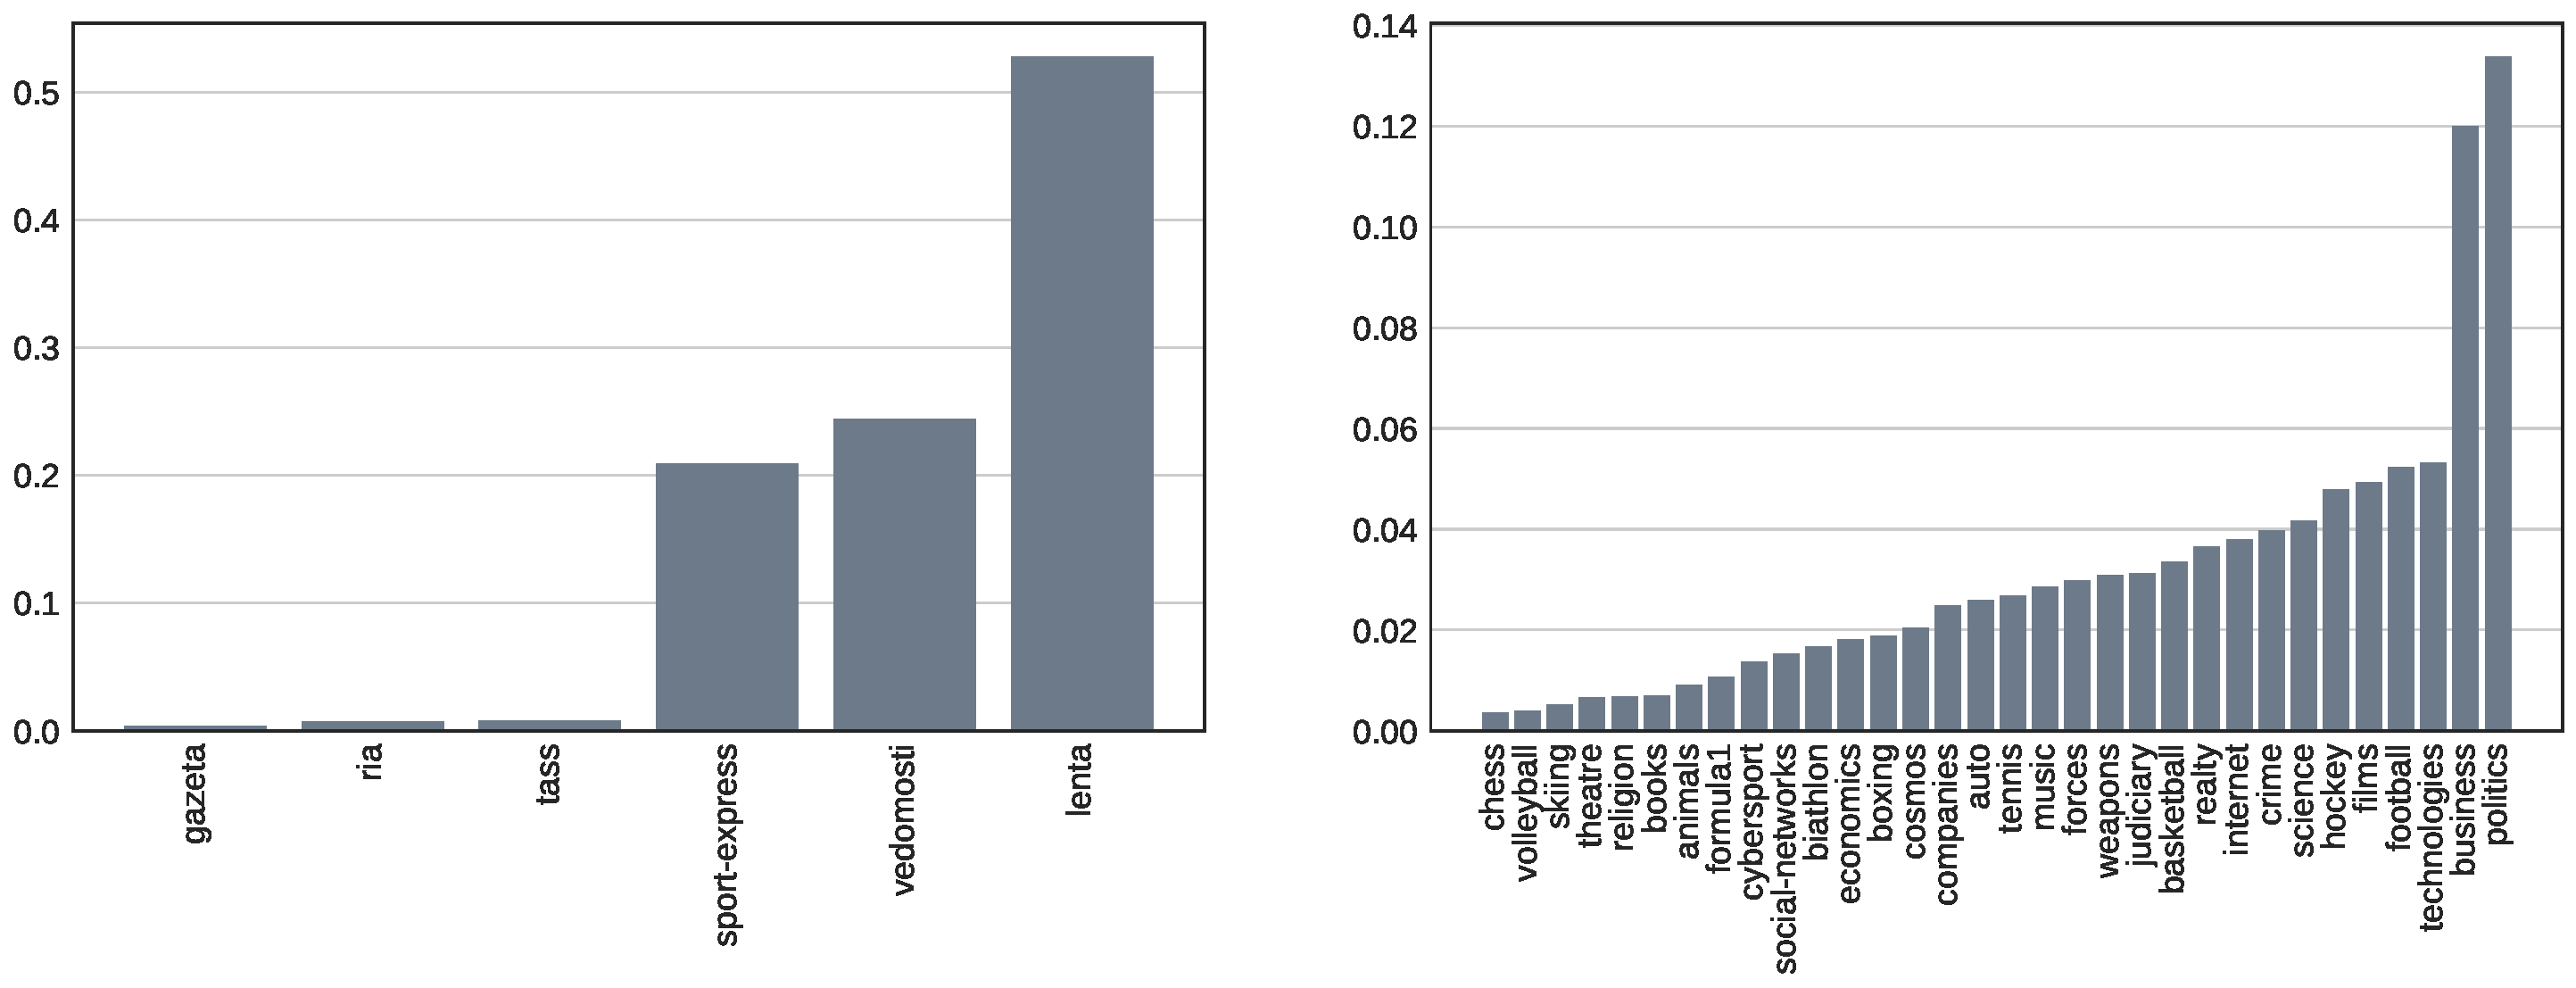
\includegraphics[width=1\textwidth]{media_topi_distr.pdf}
	\caption{Распределение СМИ и тем в данных}
	\label{media_topic_distr}
\end{figure}

%\lipsum[3-4]
%Заменил препроцессинг на нормализацию
\subsection{Нормализация новостных статей}
Нормализация является одной из важнейших стадий обработки естественного языка. Не формально, нормализация приводит текст в 
более информативный для моделей вид. В зависимости от языка процесс нормализации может отличаться. Например, для русского языка
зачастую удаляют пунктуацию и стоп-слова, а также производят лемматизацию. Стоп-слова --- это слова, которые примерно 
одинаково распределены по всему корпусу языка, чаще всего ими являются местоимения, предлоги и союзы. Лемматизация --- 
приведение слова в начальную форму (лемма):
\begin{itemize}
	\item для существительных --- именительный падеж, единственное число;
	\item для прилагательных --- именительный падеж, единственное число, мужской род;
	\item для глаголов, причастий, деепричастий --- глагол в инфинитиве.
\end{itemize}

Часто вместо лемматизации используется стемминг --- алгоритм, который убирает части 
слова, влияющие на его форму, например, окончание. В результате применения данной процедуры однокоренные слова, как правило,
преобразуются к одинаковому виду. Данные алгоритмы не только опираются на словари, но и на 
определённые правила, зависящие от языка, так как в корпусе могут встречаться слова в разных формах, которых нет в 
словаре, например, неологизмы, но образованы они по правилам языка.

Процесс обработки текста в данной работе состоит из нескольких последовательных этапов:
\begin{enumerate}
	\item Приведение текста в нижний регистр.
	\item Удаление чисел и символов пунктуации. Дефис сохраняется.
	\item Удаление стоп-слов. В данный набор входят наиболее часто употребляемые слова русского и английского языков,
	а также названия новостных агентств (<<лента>>, <<тасс>>, <<риа>> и т.д.), сохранение которых приводит к 
	переобучению моделей.
	\item Лемматизация каждого слова с помощью библиотеки MyStem\footnote{\url{https://tech.yandex.ru/mystem/}}.
\end{enumerate}
%Исходный код конвеера можно найти в приложении. %TODO: добавить ссылку

\section{Классификация новостных статей}
За последние два десятка лет, в результате активных исследований в области машинного обучения,
было изобретено множество успешных алгоритмов классификации. Например, такие модели как support vector machines (SVM) \cite{weston99svms},
градиентный бустинг над решающими деревьями и нейронные сети \cite{DBLP:journals/corr/ConneauSBL16}, были успешно применены к задачам классификации текстов.
В данной работе для классификации новостных статей использовались две из перечисленных выше модели --- это SVM и градиентный бустинг
над решающими деревьями.

Анализ текста является важной частью машинного обучения, однако сырые данные, а именно последовательности символов переменной длины,
не могут быть переданы на вход алгоритму в явном виде т.к. большинство моделей ожидают численный вектор признаков фиксированной длинны.

Векторизация --- метод трансформации коллекции текстовых документов в числовые вектора признаков.
Существуют различные подходы к векторизации текста, в данной работе были применены два самых популярных: TF-IDF и word2vec.

\subsection{Линейная модель на TF-IDF признаках}
Одним из самых простых подходов к решению задачи классификации текстовых документов является обучение линейного классификатора на
TF-IDF признаках, посчитанных на корпусе документов.

TF-IDF --- статистическая мера, используемая для оценки важности слова в контексте 
документа, являющегося частью коллекции документов или корпуса.\cite{doi:10.1108/eb026526}
TF-IDF --- это произведение двух статистик: TF (term frequency) и IDF (inverse 
document frequency). На сегодняшний день, TF-IDF один из самых популярных способов взвешивания слов, входящих в корпус документов.
Например, 83\% рекомендательных систем цифровых библиотек используют TF-IDF \cite{Beel2016}.

Существует множество способов подсчёта TF-IDF, в данной работе использовался следующий:
$$
\text{tf}(t, d) = \cfrac{n_t}{\sum_{k} n_k},
$$
где $n_{t}$ есть число вхождений слова $t$ в документ, а $\sum_{k} n_k$ --- общее число слов в данном документе.
$$
\text{idf}(t, D) = \log{ \cfrac{|D|}{|\{ d_i \in D \mid t \in d_i \}|}},
$$
где $|D|$ --- число документов в корпусе, $|\{ d_i \in D \mid t \in d_i \}|$ — число документов из коллекции $D$, в которых встречается 
$t$ (когда $n_{t} \neq 0$).

Таким образом, мера TF-IDF является произведением двух сомножителей:
$$
\text{TF-IDF}(t, d, D) = \text{tf}(t, d) \cdot \text{idf}(t, D).
$$

Признаковым описанием одного объекта $d \in D$ будет вектор
$$
\big(\text{TF-IDF}(t,d,D)\big)_{t\in V},
$$
где $V$ --- словарь всех слов, встречающихся в коллекции $D$.

Для преобразования новостных статей в числовые признаки, использовался класс \verb+TfidfVectorizer+ из библиотеки машинного обучения Scikit-learn 
\cite{scikit-learn}. В качестве параметров векторизации использовались следующие значения: \verb+min_df=3+ --- учитываются слова, встретившиеся 
суммарно во всех документах минимум 3 раза и  \verb+ngram_range=(1,2)+~--- учитываются как отдельные слова, так и би-граммы.

После векторизации новостных статей, была получена разрежённая матрица размера $133\,529$ строк на $1\,025\,919$ столбцов. По причине большого 
количества признаков ($\gg$  обучающих примеров), в качестве классификатора было решено использовать линейный SVM. Не смотря на то, что данный 
алгоритм был впервые описан более пятидесяти лет назад, сегодня он по прежнему показывает одни из самых высоких результатов в задачах классификации 
текста. Как было показано в \cite{wang12simple}, особенно высокое качество удаётся получить при использовании би-грамм.

В данной работе в качестве SVM использовался \verb+SGDClassifier+ из библиотеки Scikit-learn. Данный класс реализует различные линейные
классификаторы, параметры которых оптимизируются с помощью алгоритма стохастического градиентного спуска \cite{Bottou2010}.

Классификатор обучался со следующими параметрами: \verb+loss="hinge"+~--- функционал качества линейного SVM,
\verb+n_iter=70+~--- число итераций оптимизационного алгоритма, \verb+alpha=1e-5+~--- коэффициент регуляризации.

Обучение классификатора происходило на $70\%$ новостных статей, остальные $30\%$ использовались для валидации.
%TODO STRATIFIED
Качество классификации оценивалось с помощью метрик Accuracy и F1-меры с макро-усреднением по каждому классу.
На валидационном множестве линейному SVM удалось получить $\text{accuracy} = 0.8792$ и $\text{F1} = 0.8860$. Из матрицы ошибок,
приведённой на рисунке \ref{svm_confusion}, можно увидеть, что модель часто ошибается в классификации новостей на тему \\
<<экономика>>, относя их к новостям про <<бизнес>> (в $20\%$ случаев). Такая же ситуация характерна и для классов <<компании>>~-- 
<<бизнес>> ($12\%$), <<силовые структуры>>~-- <<оружие>> ($12\%$),  <<социальные сети>>~-- <<интернет>> ($15\%$), <<театр>>~-- 
<<кино>> ($9\%$). Перечисленные ошибки являются, в основном, причиной семантической схожести классов, но зачастую одна и та же 
новость может содержать различные темы, поэтому, возможно, нужно было решать данную задачу методами multilabel классификации, т.е. 
когда один объект может принадлежать сразу
нескольким классам. Напротив, среди всех тем выделяются несколько, которые классифицируются с высокой долей точности. Данные темы 
являются узкоспециализированными и почти не имеют пересечения с другими. В основном это виды спорта, такие как <<футбол>> (точность 
$0.99$), <<хоккей>> ($0.99$), <<формула-1>> ($1.00$), <<кибер-спорт>> ($0.98$) и т.д. Более детальные
значения метрик по каждому из классов можно найти на графике \ref{svm_classif_report}.

Веса признаков в линейной модели в случае, если признаки отмасштабированы, характеризуют степень их влияния на значение целевой 
переменной. В задаче классификации текстов, кроме того, признаки являются хорошо интерпретируемыми, поскольку каждый из них 
соответствует конкретному слову, поэтому из линейного SVM были извлечены слова с наибольшим весом для каждой из 32-ух тем (таблица \ref{table:svm_topwords}). 
%Для определения этих метрик, введём следующие обозначения:
%
%TP (true postive)~--- число истинно-положительных значений.
%
%TN (true negative)~--- число истинно-отрицательных значений.
%
%FP (false positive)~--- число ложно-положительных значений.
%
%FN (false negative)~--- число ложно-отрицательных значений.
%
%$\text{precision (точность)} = \cfrac{TP}{TP + FP}$ --- насколько можно доверять классификатору.
%
%$\text{recall (полнота)} = \cfrac{TP}{TP + FN}$ --- как много объектов класса 1 находит классификатор.
%
%Тогда accuracy --- доля корректно классифицированных новостных статей от общего числа статей:
%$$
%\text{accuracy} = \cfrac{\text{TP} + \text{TN}}{\text{TP} + \text{TN} + \text{FP} + \text{FN}}.
%$$
%
%F1-мера --- гармоническое среднее точности и полноты
%$$
%\text{F1} = \cfrac{2 \cdot (\text{precision} \cdot \text{recall})}{\text{precision} + \text{recall}}.
%$$

\subsection{Градиентный бустинг над решающими деревьями. Word2Vec и тематическое моделирование.}
Другим популярным подходом к векторизации текста является алгоритм Word2Vec.
Реализация алгоритма опубликованная компанией Google \cite{DBLP:journals/corr/abs-1301-3781} в 2013 году,
основывается на однослойной нейронной сети, которая пытается <<выучить>> векторные представления слов (англ. word embeddings).
До этого также были предложены различные архитектуры рекуррентных нейронных сетей, которые могли <<выучивать>> векторные 
представления, но их проблема заключалась в том, что они требовали намного больше времени для обучения, в отличии от реализации 
Word2Vec от Google.

Алгоритм Word2Vec является подмножеством более широкого класса алгоритмов, которые называются Vector space models (VSMs) 
\cite{Salton:1975:VSM:361219.361220}. VSMs представляют слова в непрерывном векторном пространстве, где семантически похожие
слова отображаются в близкие точки. VSMs имеют долгую и богатую историю в NLP, но все представители этого семейства моделей 
опираются на дистрибутивную семантику, которая утверждает, что слова появляющиеся в одном и том же контексте имеют близкое 
семантическое значение. Все методы основанные на данной гипотезе можно разделить на два класса: статистические или численные (от 
англ. count-based, пр. Latent Semantic  Analysis) и предиктивные модели (пр. neural probabilistic language models).

Первый класс алгоритмов вычисляет как часто слова возникают в контексте своих соседей в больших корпусах текстов. Затем происходит 
отображение вычисленных статистик в вектора для каждого слова. В свою очередь, предиктивные модели напрямую пытаются предсказать 
слова по его контексту, <<выучивая>> вектора таким образом, чтобы снизить ошибку предсказаний.

В частности, Word2Vec является вычислительно-эффективной реализацией предиктивной модели, которая <<выучивает>> векторные 
представления слов из необработанных текстовых данных. Есть две вариации алгоритма: Continuous Bag-of-Words (CBOW) и Skip-Gram. 
Алгоритмически они  похожи, за  исключением того, что CBOW предсказывает слово (например <<раму>>) основываясь на контексте (<<мама 
мыла>>), в то время как Skip-Gram наоборот, старается предсказать контекст по исходному слову. На практике CBOW лучше работает на 
небольших корпусах текстов, однако если  корпус достаточно большой, как в данной работе, то рекомендуется использовать модель, 
основанную на Skip-Gram.

В данной работе, для обучения модели Word2Vec использовалась библиотека Gensim \cite{rehurek_lrec}, в которой имеется обёртка над 
Word2Vec от Google  для языка Python. Модель обучалась в течении 50 минут со следующими параметрами: \verb|min_count=3|~--- в 
обучении используются только те слова,  которые встречаются во всём корпусе не менее трёх раз, \verb|vec_size=300|~--- размерность 
векторов слов, \verb|window=5|~--- размер окна (контекста), \verb|sg=1|~--- использовать алгоритм Skip-Gram, \verb|iter=10|~--- 
количество итераций по коллекции документов.

Результатом обучения Word2Vec является словарь, который отображает слова в вектора. Для представления новостной статьи в виде 
вектора признаков усредним все векторы слов в данной статье с idf весами. В результате получим матрицу, в которой $133\,529$ строк 
и $300$ столбцов (признаков), что значительно меньше, чем в случае TF-IDF. Благодаря тому, что удалось снизить размерность с 
$1\,025\,919$ признаков до $300$, становится возможным эффективное использование таких мощных алгоритмов как градиентный бустинг 
над решающими деревьями.

Градиентный бустинг над решающими деревьями --- один из самых универсальных и сильных методов машинного обучения, известных
на сегодняшний день. В последнее время этот алгоритм и, особенно его реализация в библиотеке XGBoost 
\cite{DBLP:journals/corr/ChenG16}, пользуются большой популярностью у участников соревнований в области анализа данных на платформе 
Kaggle.

В данной работе использовалась реализация градиентного бустинга из библиотеки LightGBM, которая является open-source проектом компании
Microsoft. Алгоритм построения деревьев в LightGBM немного отличается от того, как это реализовано в XGBoost. Несмотря на это интерфейс библиотек
и параметры алгоритмов зачастую полностью совпадают. Однако на практике LightGBM превосходит в скорости работы XGBoost, именно по этой причине
эта библиотека использовалась для решения задачи классификации.

Модель градиентного бустинга над деревьями обучалась на векторах, полученных с помощью Word2Vec, в течении 26 минут, со следующими параметрами:
\begin{enumerate}
	\item \verb|colsample_bytree=0.9| --- доля от общего числа признаков, используемая для построения дерева на каждой итерации;
	\item \verb|learning_rate=0.1| --- шаг градиентного спуска, темп обучения;
	\item \verb|max_depth=7| --- ограничение на максимальную глубину дерева;
	\item \verb|num_leaves=255| --- ограничение на максимальное число листьев в дереве;
	\item \verb|objective="multiclass"| --- функционал качества;
	\item \verb|metric="multi_error"| --- метрика, по которой оценивается качество и происходит ранняя остановка;
	\item \verb|subsample=0.8| --- доля от общего числа объектов, используемых для построения дерева на каждой итерации.
\end{enumerate}
Итоговое качество алгоритма: $\text{Accuracy} = 0.8427$, $\text{F1} = 0.8486$.

Как видно из результатов, качество градиентного бустинга оказалось ниже линейного SVM, что, возможно, является причиной усреднения слов в документе,
во время которого теряется достаточно много информации. Одним из решений данной проблемы является генерация новых признаков. Для этого 
в работе было применено тематическое моделирование.

Тематическое моделирование --- активно развивающаяся ветвь статистического анализа текстов \cite{Blei:2012:PTM:2133806.2133826}. Тематические
модели стараются раскрыть скрытую тематическую структуру коллекции документов и найти сжатое представление каждого документа в виде
тем, которые в нём встречаются. Тематическое моделирование применяется в различных задачах, например, таких как информационный поиск,
классификация, кластеризация, сжатие текста без потери информации (summarization) и т.д. Различные способы и идеи применения тематических моделей
описаны в обзоре \cite{Daud2010}.

Статистически, модель вероятностного тематического моделирования определяет каждую тему как многомерное распределение над словами
$P\left(w \,\middle|\, t\right)$, где $w$~--- слово, $t$~--- тема, и затем описывает каждый документ в виде многомерного распределения тем $P\left(t \,\middle|\, d\right)$, где $d$~--- документ. Тематическая модель выявляет скрытые темы по наблюдаемым распределениям слов 
$P\left(w \,\middle|\, d\right)$ в документах.

В данной работе для тематического моделирования использовалась библиотека bigARTM \cite{bigartm} --- открытая библиотека для тематического 
моделирования текстовых коллекций, реализующая теорию аддитивной регуляризации тематических моделей (ARTM).

\section{Агрегация новостных статей}
В данной работе, в качестве меры семантической схожести двух новостей, используется косинусная мера.
Пусть есть две новости, которые представлены в виде двух векторов $x$ и $y$. Известно, что их скалярное произведение
и косинус угла $\alpha$ между ними связаны следующим соотношением:
$$
\langle x,y \rangle = \Vert x \Vert \Vert y \Vert \cdot \cos(\alpha).
$$
Тогда, косинусное расстояние определяется как
$$
\rho_{\cos}(x, y) = \arccos\left(\frac{\langle x,y \rangle}{\Vert x \Vert \Vert y \Vert} \right).
$$

Косинусное расстояние часто используется для измерения схожести между текстами.
Каждый документ описывается вектором, каждая компонента которого соответствует слову из словаря. В данной работе, компонента
вектора --- это TF-IDF вес слова, если оно встречается в тексте, и ноль в противном случае.
Тогда косинус между двумя векторами будет тем больше, чем больше общих слов в этих двух документах одновременно.

После кластеризации кластеры сортируются по убыванию среднего времени новостей в них. Это необходимо для того, чтобы новые
статьи отображались выше старых.

\subsection{Кластеризация с помощью алгоритмов машинного обучения}

\subsection{Объединение в связные компоненты графа}
Данный алгоритм основан на алгоритме нахождения связных компонент в графе. Изначально строится полный граф,
где вершины~--- векторное представление новостей, а вес рёбер равен косинусному расстоянию между вершинами.
Рёбра, вес которых меньше определённого параметра, игнорируется, и запускается алгоритм поиска в ширину
от первой вершины, не находящейся в кластере. Все вершины, по которым прошёл поиск, добавляются
в кластеры и помечаются как посещённые, и начинается новый поиск от следующей непомеченной вершины.
Такой поиск производится до тех пор, пока все вершины не станут находится в каком-либо кластере.

\section{Разработка веб-приложения}
Веб-приложение состоит из двух основных частей: back-end и front-end. Back-end -- это сам веб-сервер,
который осуществляет обработку запросов пользователей, получение и обработку данных.
Front-end -- это пользовательский интерфейс, визуализирующий полученные от back-end данные в понятный вид.
С помощью этого интерфейса пользователь способен не только получать, но и передавать данные на back-end.

Back-end составляющая сервиса реализована на языке Python 3, с использованием библиотек: Flask~---
обрабатывает HTTP запросы от пользователей, pandas~--- обработка и хранение данных; sklearn~--- модели TFIDF, KMeans, SVM;
pymystem3~--- лемматизация.

Структура приложения показана на рис. \ref{server_struct}.

\begin{figure}[h]
    \centering
    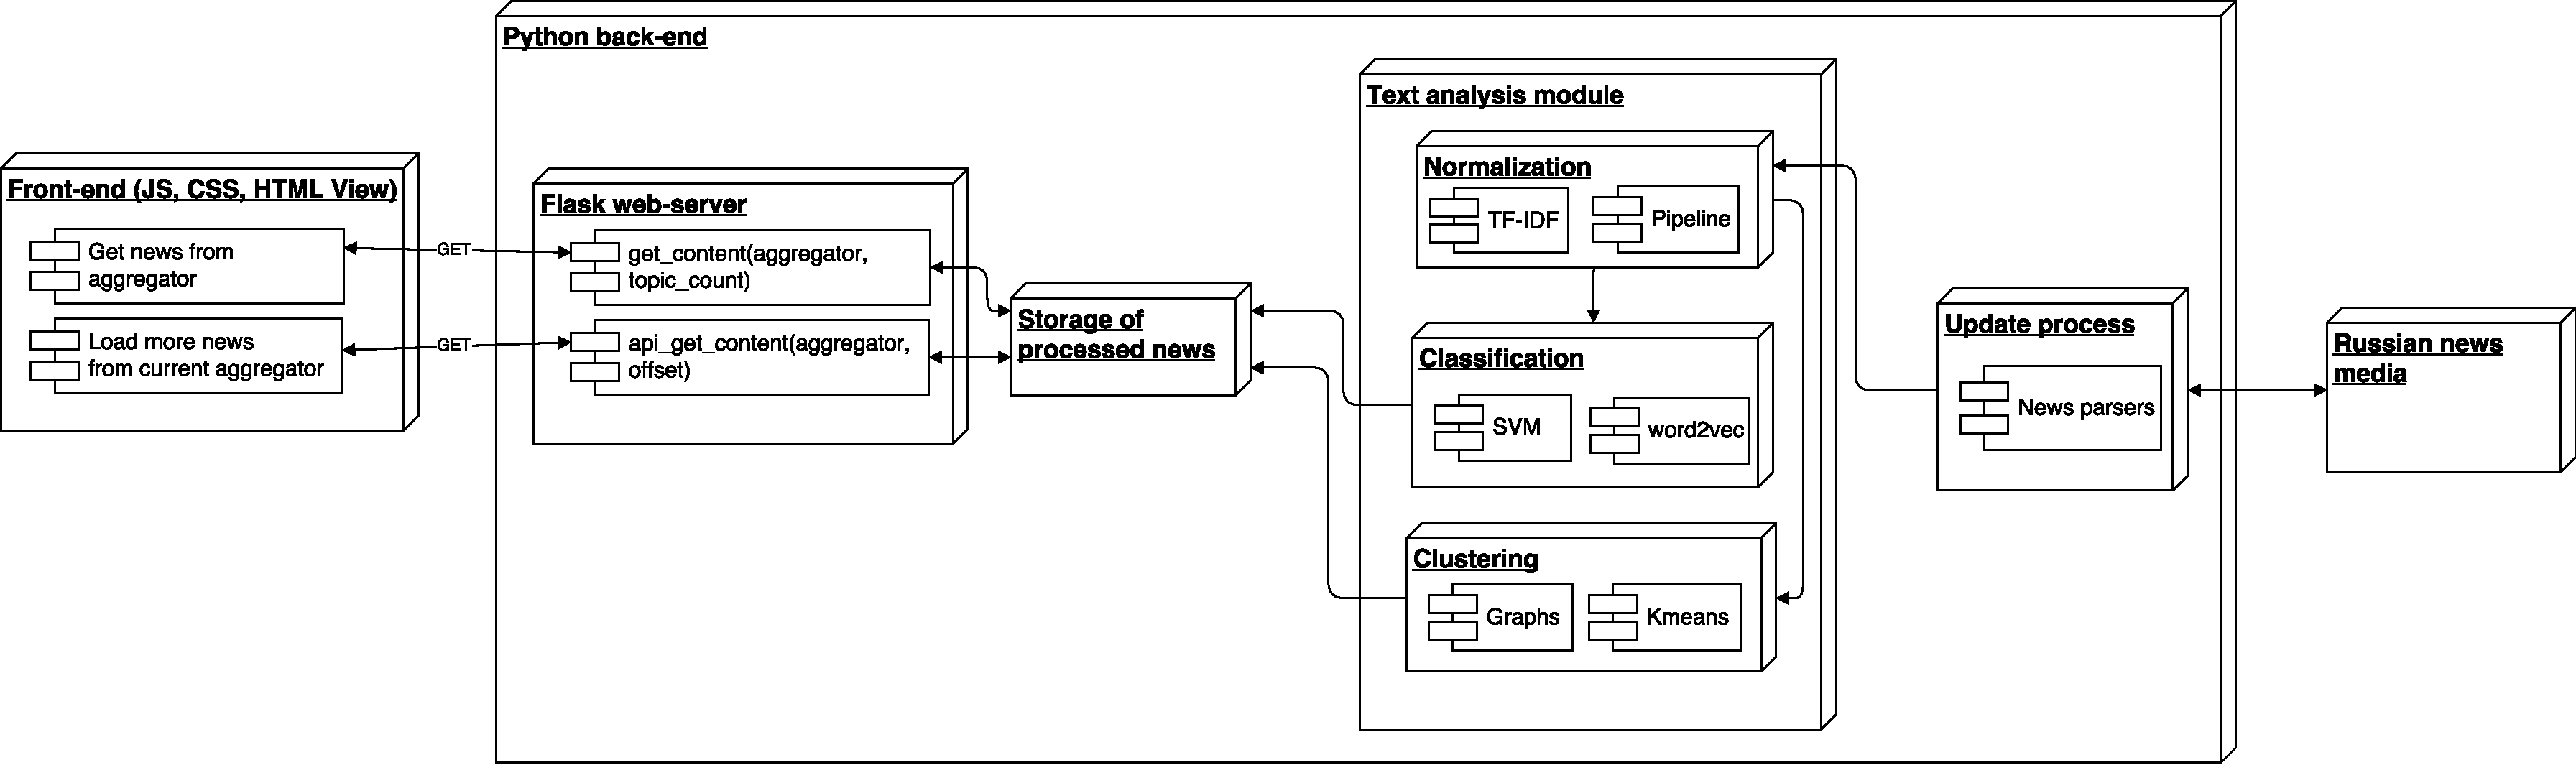
\includegraphics[width=1\textwidth]{server_infrastructure.pdf}
    \caption{Структура сервера}
    \label{server_struct}
\end{figure}

Back-end разделён на несколько модулей: Flask web-сервер, модуль парсеров новостей, которые
с помощью параллельных процессов извлекают данные с сайтов СМИ, модуль анализа данных.

При запуске сервера происходит получение новостей за последние 12 часов и их обработка.
После этого запускается отдельный процесс, отвечающий за актуальность данных: каждую минуту он
проверяет наличие новых статей, и, если такие есть, отправляет их на обработку. При запросе от Front-end, сервер
обращается к уже обработанным данным, хранящимся в кэше.

Основной частью сервера является класс Analizer, обрабатывающий полученные
новостные статьи.

Методы класса:
\begin{itemize}
    \item \verb|Конструктор|. Параметры: список новостных статей с мета-данными.

    В конструкторе класса производится загрузка сохраненных моделей, определяются параметры моделей агрегации, вызываются функции 
    функции \verb|_data_to_pandas|, \verb|_classify|, \verb|_classify|, \verb|_aggregate|, \verb|_form_output|.

    \item \verb|append_data|. Параметры: список новостных статей с мета-данными.

    Функция отвечает за добавление новых данных. Вызываются те же методы, что и
    в конструкторе. Дополнительно удаляются устаревшие данные.

    \item \verb|_data_to_pandas|. Параметры: список новостных статей с мета-данными. Возвращаемое значение: \verb|Pandas Dataframe|, в котором хранится
    вся информация о актуальных новостях.

    Список новостей конвертируется в таблицу \verb|Pandas Dataframe|, из которой
    удаляются дубликаты, лишние мета-данные, происходит сортировка по дате 
    публикации статьи. Вызывается функция \verb|_norimalize|.

    \item \verb|_norimalize|. Параметры: \verb|Pandas Dataframe|.

    Вызываются конвеер с функциями нормализации. К таблице
    добавляются нормализованные текст и заголовок статей.

    \item \verb|_classify|. Параметры: \verb|Pandas Dataframe|.

    Вызываются функции классификации. Для каждого классификатора реализована отдельная функция, в которой к таблице добавляются колонка с тегами,
    полученными от данного классификатора.

    \item \verb|_aggregate|. Параметры: \verb|Pandas Dataframe| и 
    конфигурация агрегаторов.

    Вызываются функции агрегации: \verb|_aggregate_Kmeans|,
    \verb|_aggregate_graphs|.

    Для каждого агрегатора реализована отдельная функция, которые возвращают список кластеров, каждый кластер представляет
    собой список ID --- индекс новости в таблице \verb|Pandas Dataframe|.

    \item \verb|_sort_groups|. Параметры: список кластеров, полученный от
    агрегаторов. Возвращает отсортированный список кластеров.

    Фильтрует кластеры, в которых меньше двух новостей, сортирует кластеры по среднему времени публикации, и сортирует новости внутри кластера по времени.

    \item \verb|_get_avg_time|. Параметры: кластер. Возвращает среднее время
    в кластере.

    Преобразовывает даты публикации каждой новости класстера в Unix-секунды и
    считает от них среднее.

    \item \verb|_get_TFIDF|. Параметры: \verb|Pandas Dataframe|.
    Возвращает модель TF-IDF и матрицу векторизованных новостей.

    \item \verb|_class_to_str|. Параметры: id класса.
    Возвращает название класса.

    \item \verb|_cut_text|. Параметры: текст.
    Возвращает первый абзац текста.

    \item \verb|_date_to_str|. Параметры: дата публикации.
    Возвращает дату в виде строки в определённом формате.

    \item \verb|_form_output|. Параметры: \verb|Pandas Dataframe|, список
    кластеров.

    Формирует данные в формате JSON, используемым веб-сервером, и сохраняет их.

    \item \verb|get_data|. Параметров нет.
    Возвращает готовые данные в формате JSON, используемы веб-сервером, и
    дату самой актуальной новости.

\end{itemize}
% \subsection{Back-end часть}
% \subsection{Front-end часть}

\section{Заключение}

\bibliography{biblio}
 % Список литературы

\setcounter{secnumdepth}{0}
\section{Приложение}
\begin{figure}[h!]
	\centering
	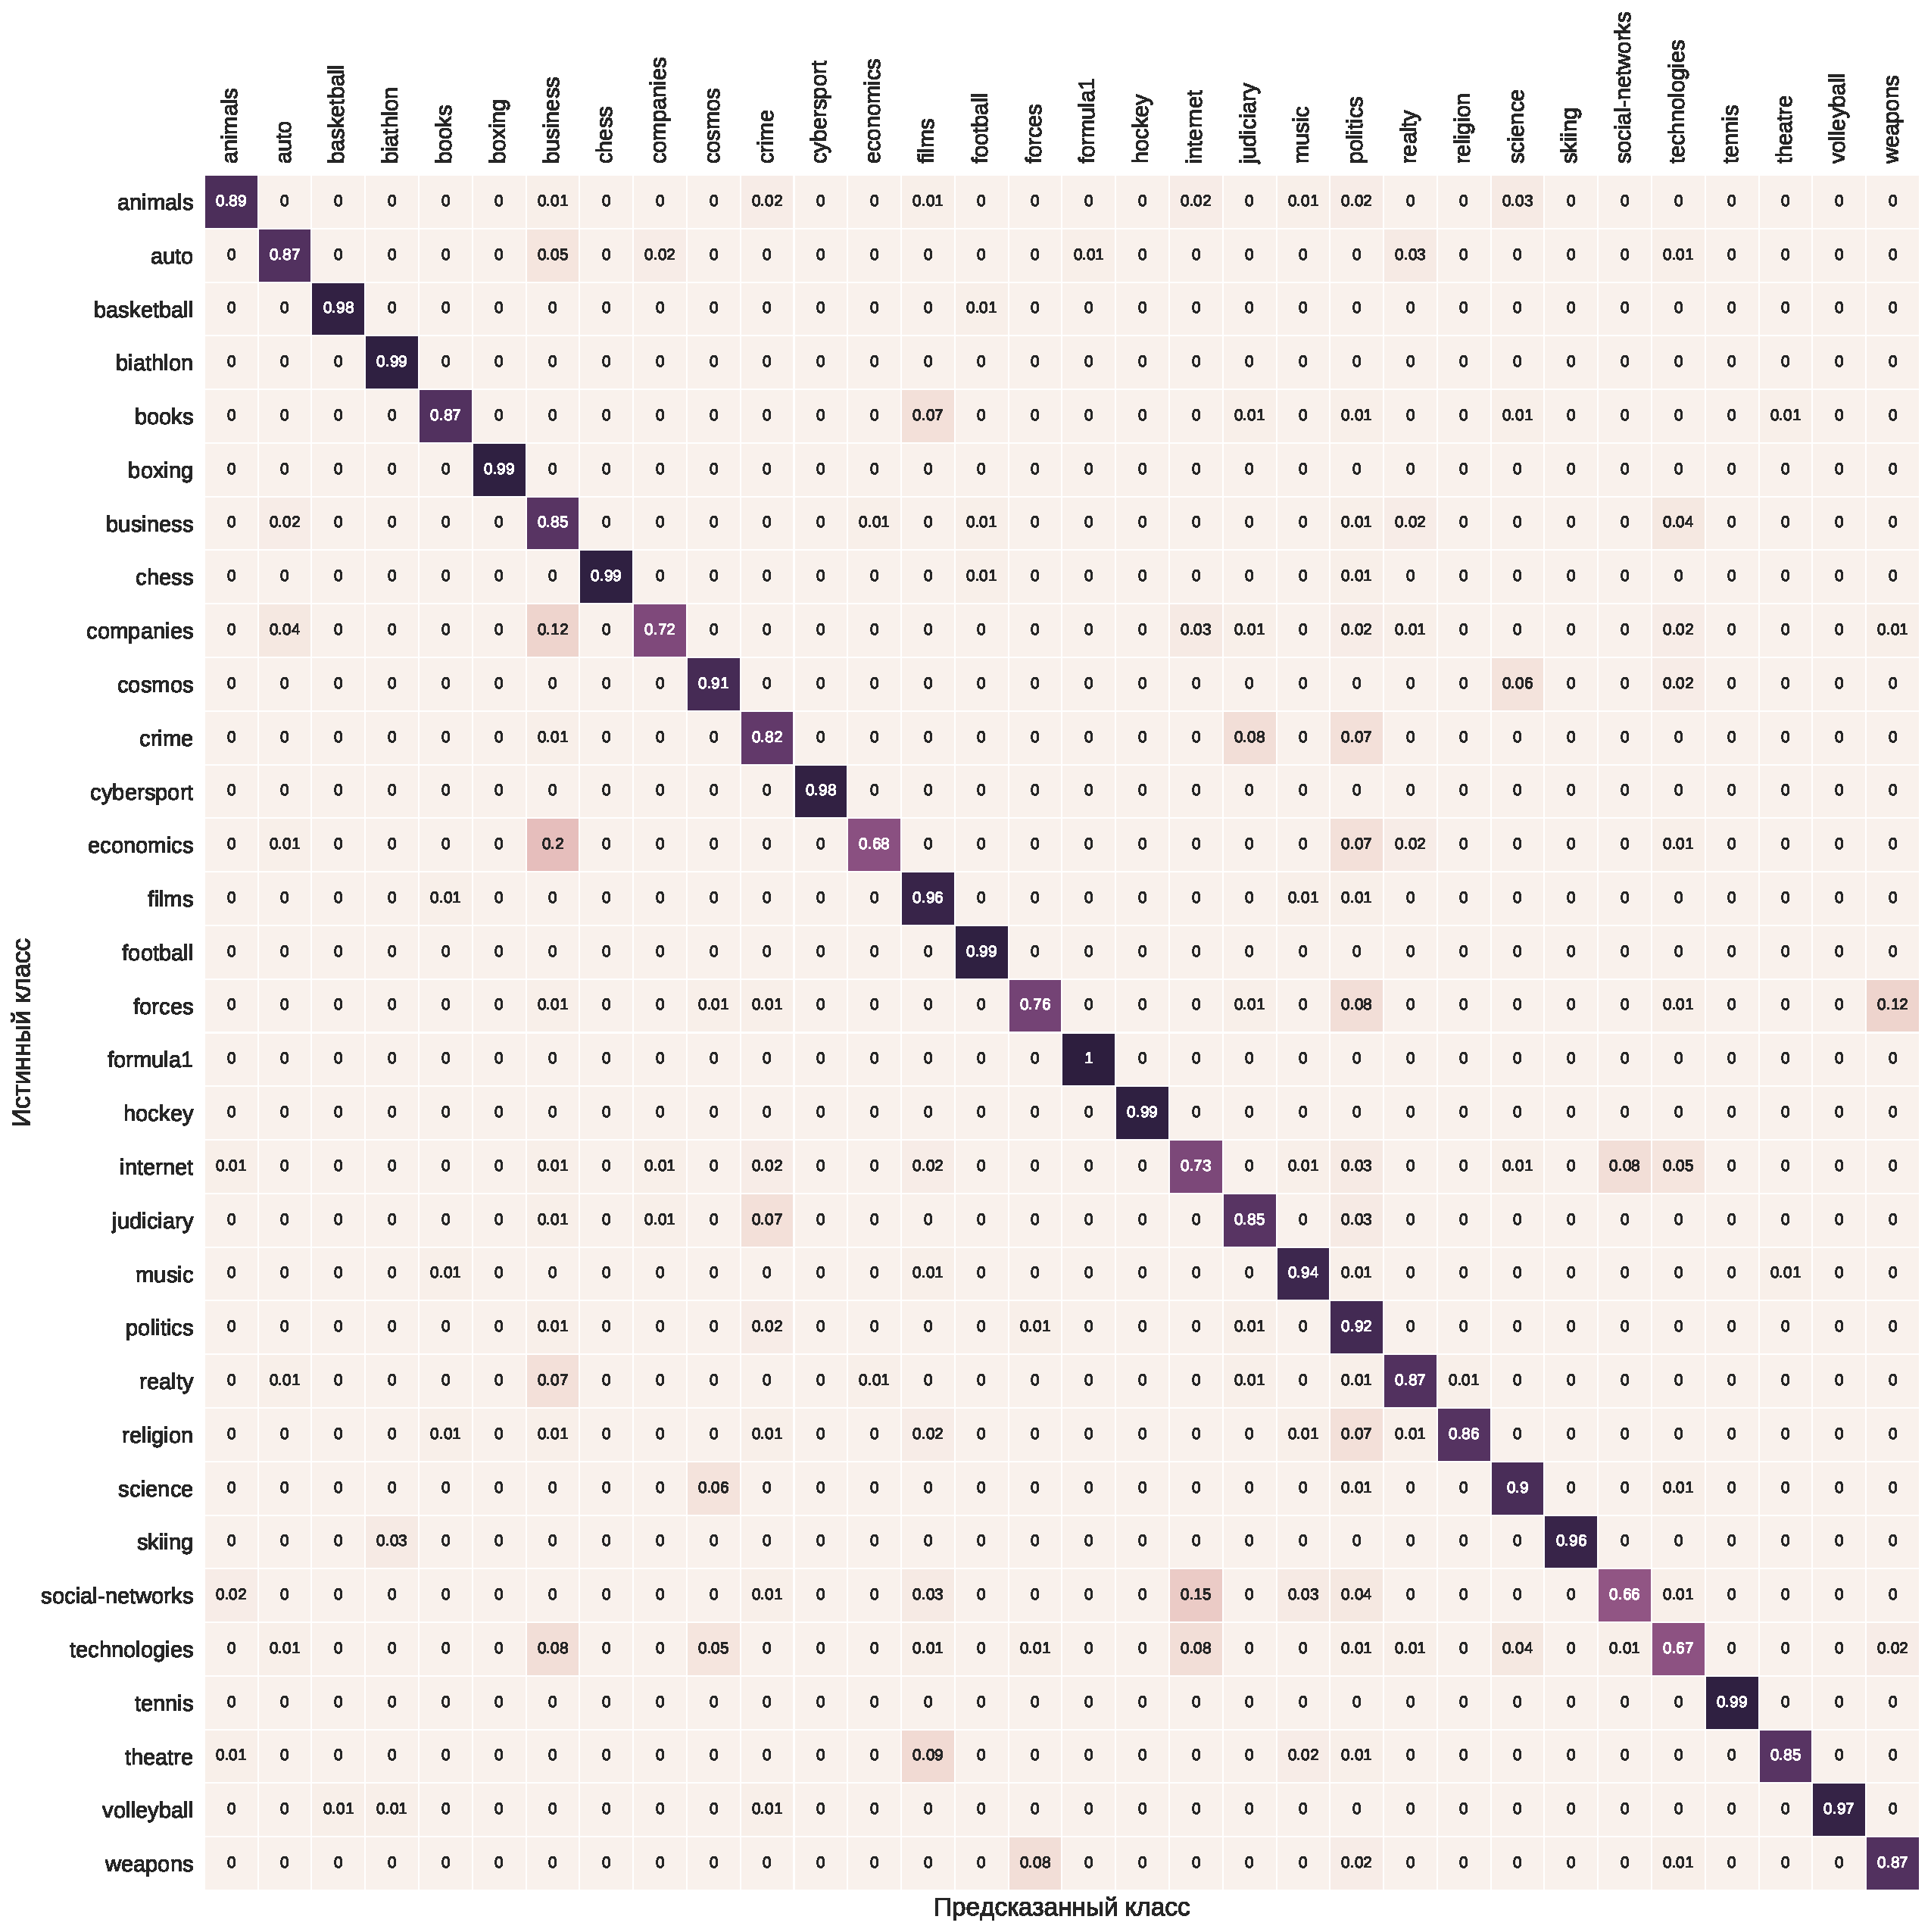
\includegraphics[width=1\textwidth]{svm_confusion_matrix.pdf}
	\caption{Матрица ошибок линейного SVM}
	\label{svm_confusion}
\end{figure}

\begin{figure*}[t!]
	\centering
	\begin{subfigure}[t]{0.5\textwidth}
		\centering
		\hspace*{-2cm}
		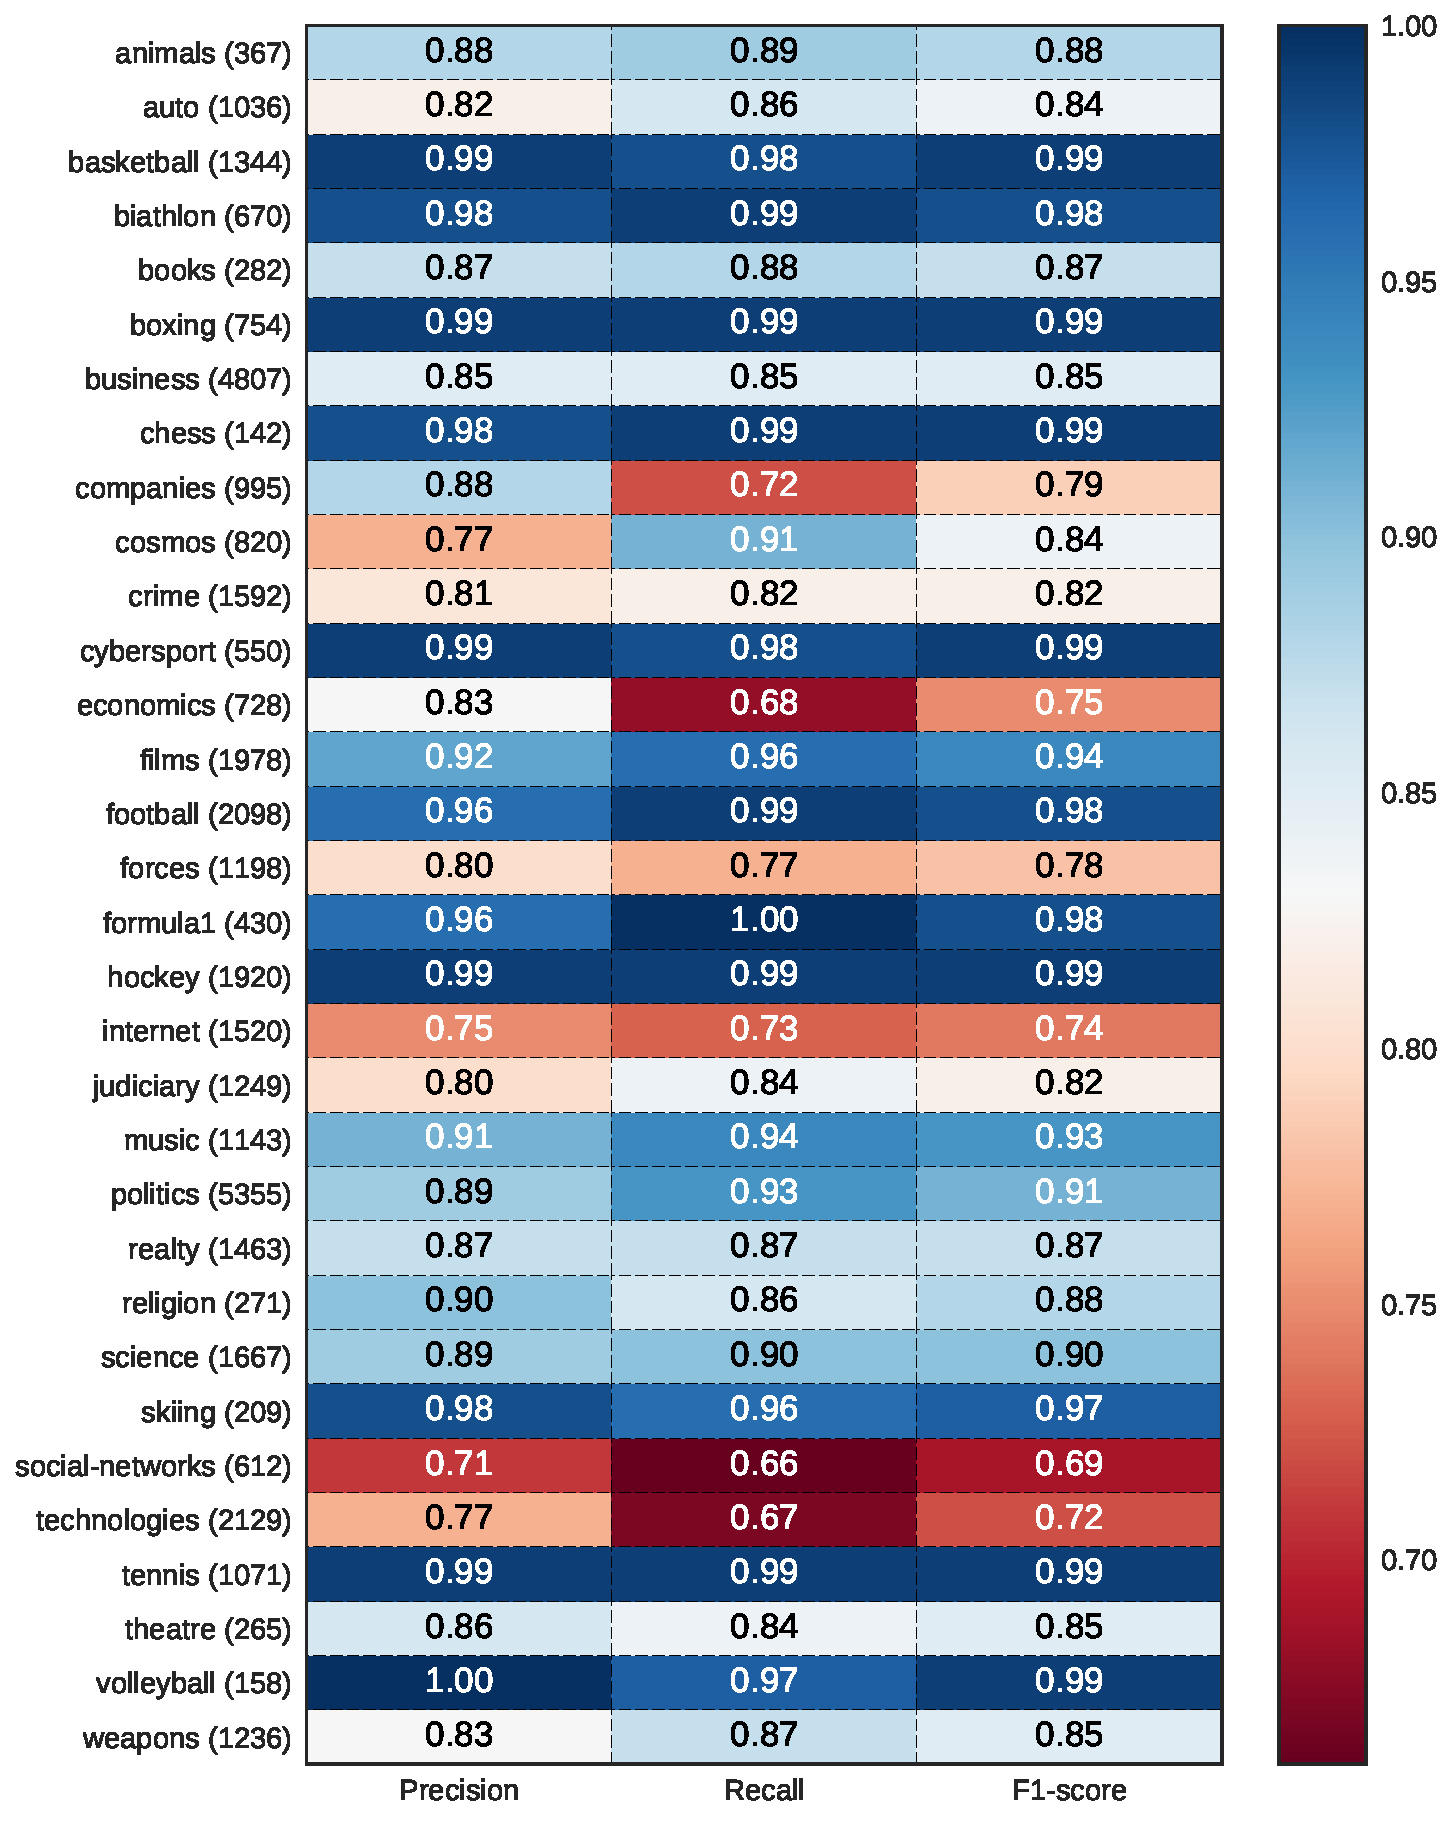
\includegraphics[width=1\textwidth]{svm_classif_report.pdf}
		\caption{Линейный SVM}
		\label{svm_classif_report}
	\end{subfigure}%
	~ 
	\begin{subfigure}[t]{0.5\textwidth}
		\centering
		\hspace*{-2cm}
		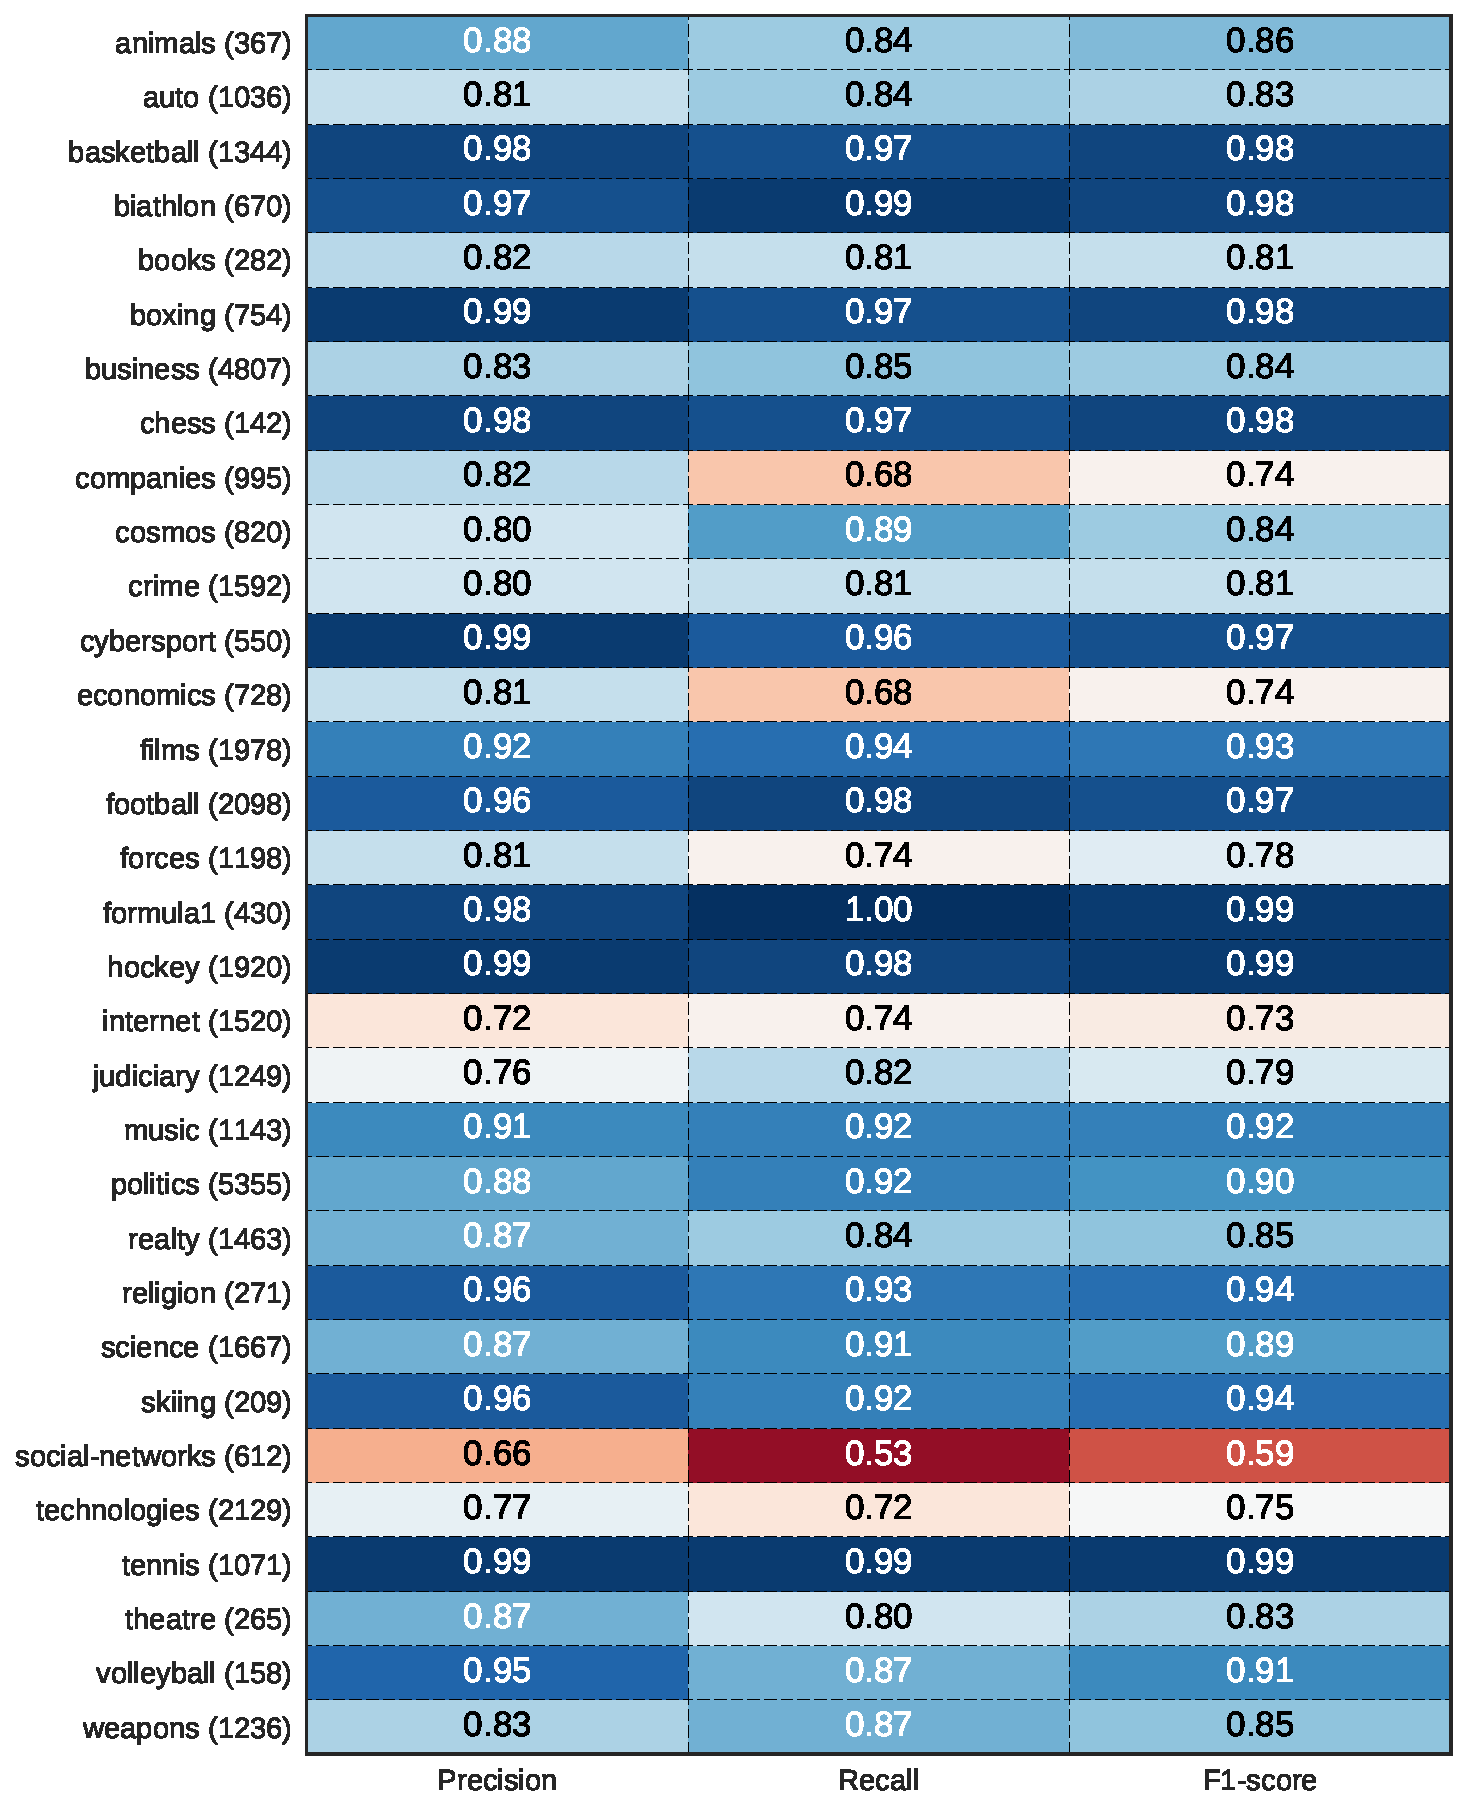
\includegraphics[width=1\textwidth]{lgb_w2v_bigartm_classif_report.pdf}
		\caption{LightGBM + Word2Vec + bigARTM}
	\end{subfigure}
	\caption{Precision, Recall и F1 мера по каждому из классов}
\end{figure*}

\begin{table}[h]
	\resizebox{\textwidth}{!}{%
		\begin{tabular}{r|cccccccc}
			\toprule
			\textbf{animals}         &               жить &          вольер &             хозяин &              животный &               зоопарк &        питомец &           кличка &        животное \\
			\textbf{auto}            &          авторынок &           осаго &      автомобильный &     автопроизводитель &              автопром &          камаз &          автоваз &      автомобиль \\
			\textbf{basketball}      &                рфб &      евробаскет &          центровой &          кубок европа &             баскетбол &   баскетболист &         евролига &             нба \\
			\textbf{biathlon}        &           эстафета &    биатлонистка &            шипулин &                   сбр &            хохфильцен &        биатлон &              ibu &      биатлонист \\
			\textbf{books}           &         библиотека &    произведение &       писательница &                 роман &                 книга &   литературный &             поэт &        писатель \\
			\textbf{boxing}          &              алоян &          лебзяк &                мма &              поединок &              поветкин &            бой &             бокс &          боксер \\
			\textbf{business}        &   россельхознадзор &            fifa &                ржд &               газпром &           туроператор &        formula &         ритейлер &             оао \\
			\textbf{chess}           &            карякин &       шахматист &           карякина &                магнус &               шахматы &        карлсен &              фид &       шахматный \\
			\textbf{companies}       &  тысяча автомобиль &        компания &  миллиард кубометр &              миллиард &                тысяча &  процент акция &         ретейлер &         процент \\
			\textbf{cosmos}          &          космонавт &         светить &           прогресс &             вселенная &                космос &     астрофизик &             марс &       астронавт \\
			\textbf{crime}           &          грабитель &         изымать &        группировка &               полиция &               убивать &         летний &       преступник &          тюрьма \\
			\textbf{cybersport}      &             gaming &            team &              valve &           киберфутбол &                  dota &     киберспорт &  киберспортивный &  киберспортсмен \\
			\textbf{economics}       &               мрот &          греция &             бюджет &                пенсия &                   ввп &         минфин &        экономика &        инфляция \\
			\textbf{films}           &         мультфильм &          сериал &            актриса &                  кино &               картина &       режиссер &            актер &           фильм \\
			\textbf{football}        &               поле &         стадион &         нападающий &              матч тур &                  фифа &           уефа &        футболист &    полузащитник \\
			\textbf{forces}          &       развертывать &      выполнение &     военнослужащий &               военный &                 шойгу &        генштаб &       конашенков &      минобороны \\
			\textbf{formula1}        &              манор &      цитировать &               рено &               феррари &              макларен &          пилот &         мерседес &         формула \\
			\textbf{hockey}          &           авангард &             ска &              шайба &            нападающий &                хоккей &       хоккеист &              нхл &             кхл \\
			\textbf{internet}        &          википедия &          сервис &             ресурс &               youtube &                  сайт &          хакер &           блогер &        интернет \\
			\textbf{judiciary}       &             стража &          статья &       арестовывать &               колония &  следственный комитет &      следствие &              скр &  комитет россия \\
			\textbf{music}           &         композитор &     евровидение &              песня &                 певец &               концерт &         альбом &           певица &        музыкант \\
			\textbf{politics}        &              лидер &          кремль &      парламентарий &                партия &               депутат &        госдума &            глава &             мид \\
			\textbf{realty}          &             объект &    строительный &           жилищный &         строительство &                   жкх &        ипотека &            жилье &    недвижимость \\
			\textbf{religion}        &          монастырь &           собор &          церковный &                муфтий &                святой &       христиан &       митрополит &        патриарх \\
			\textbf{science}         &        университет &          журнал &          математик &                 физик &               научный &       археолог &    исследователь &          ученый \\
			\textbf{skiing}          &             вяльбе &          нортуг &             лыжник &                   fis &                легков &         йохауг &            лахти &         устюгов \\
			\textbf{social-networks} &          некоторые &            юзер &           facebook &               twitter &     пользователь сеть &   пользователь &        вконтакте &         соцсеть \\
			\textbf{technologies}    &          vimpelcom &           apple &           оператор &                  wifi &              говорить &            мтс &            робот &         контакт \\
			\textbf{tennis}          &    кубок федерация &            open &            шарапов &                теннис &                  корт &      теннисист &      теннисистка &     кубок дэвис \\
			\textbf{theatre}         &         росгосцирк &        цирковой &              балет &            постановка &           театральный &         мюзикл &            театр &       спектакль \\
			\textbf{volleyball}      &              факел &         маричев &             алекно &             суперлига &             казанский &      белогорье &      волейболист &        волейбол \\
			\textbf{weapons}         &               jane &  использоваться &       defense news &  министерство оборона &             миллиметр &  миллиметровый &          defense &             тип \\
			\bottomrule
	\end{tabular}}
	\caption{Слова с наибольшим весом по каждой теме (веса линейного SVM)}
	\label{table:svm_topwords}
\end{table}

\end{document}